\documentclass{standalone}
\usepackage{tikz}
\usepackage{ctex,siunitx,ninecolors}
\setCJKmainfont{Noto Serif CJK SC}
\usepackage{tkz-euclide}
\usepackage{amsmath}
\usepackage{wasysym}
\usetikzlibrary{patterns, calc}
\usetikzlibrary{decorations.pathmorphing, decorations.pathreplacing, decorations.shapes,3d}
\begin{document}
\small
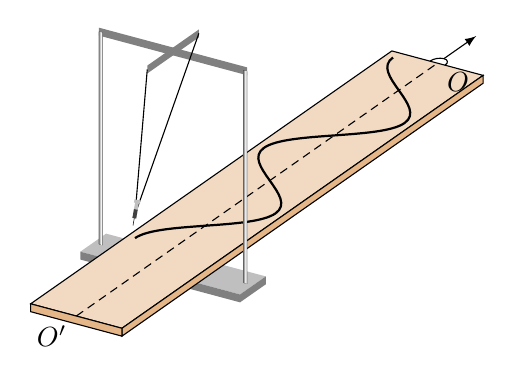
\begin{tikzpicture}[>=latex,z={(35:10mm)},x={(-15:5mm)}]
  \def\wave{
  \draw[thick,fill opacity=.2]
  (1.5,-1) cos (2,0)
  sin (2.5,1) cos (3,0) sin (3.5,-1) cos (4,0)
  sin (4.5,1) cos (5,0) sin (5.5,-1);
  }
\begin{scope}[canvas is zx plane at y=-0.2]
  \fill[lightgray](1.3,2.1)rectangle(1.7,-2.1);
\end{scope}
\begin{scope}[canvas is xy plane at z=1.3]
  \fill[gray](-2.1,-0.2)rectangle(2.1,-0.3);
\end{scope}
\begin{scope}[canvas is yz plane at x=0]
  \fill[gray](2.55,1.5)rectangle(2.45,1.9);
\end{scope}
\begin{scope}[canvas is xy plane at z=1.5]
  \fill[gray](-1.95,2.55)rectangle(1.95,2.45);
  \fill[left color=gray,right color=gray,middle color =white](-1.95,-0.2)rectangle(-1.85,2.5);
\end{scope}
\begin{scope}[canvas is yz plane at x=0]
  \fill[gray](2.55,1.5)rectangle(2.45,1.1);
\end{scope}
\begin{scope}[canvas is zx plane at y=0]
  \draw[fill=brown9](0,-1.2)rectangle(5.6,1.2);
  \draw[densely dashed](0,0)node[below left]{$O'$}--(5.6,0)node[below right]{$O$};
  \draw(5.6,0.2)arc(90:-90:0.1 and 0.2);
  \draw[->](5.7,0)--++(0.5,0);
  \wave
\end{scope}
\begin{scope}[canvas is yz plane at x=1.2]
  \draw[fill=brown8](0,0)rectangle(-0.1,5.6);
\end{scope}
\begin{scope}[canvas is yz plane at x=2.1]
  \fill[gray](-0.2,1.3)rectangle(-0.3,1.7);
\end{scope}
\begin{scope}[canvas is xy plane at z=1.5]
  \fill[left color=gray,right color=gray,middle color =white](1.95,-0.2)rectangle(1.85,2.5);
\end{scope}
\begin{scope}[canvas is xy plane at z=0]
  \draw[fill=brown8](-1.2,0)rectangle(1.2,-0.1);
\end{scope}
\draw[thin](0,2.5,1.1)--(-1,0.3,1.5)--(0,2.5,1.9);
\begin{scope}[very thin,xshift=0.72cm,yshift=1.15cm,rotate=-10]
  \draw(0,0)--(0,0.1);
  \fill[lightgray](0.05,0.1)rectangle(-0.05,0.3);
  \fill[lightgray](0.08,0.3)rectangle(-0.08,0.32);
  \fill[darkgray](0.05,0.1)rectangle(-0.05,0.2);
\end{scope} 
\end{tikzpicture}
\end{document}